\documentclass[12pt,a4paper]{article}

% ── 字体与编码 ────────────────────────────────────────────────────────────────
\usepackage{fontspec}
\usepackage{xeCJK}
\setCJKmainfont[BoldFont=SimHei]{SimSun}
\setmainfont{Times New Roman}

% ── 页面布局 ─────────────────────────────────────────────────────────────────
\usepackage[top=2.5cm,bottom=2.5cm,left=2.8cm,right=2.8cm,headheight=15pt]{geometry}
\usepackage{setspace}
\onehalfspacing

% ── 颜色主题 ─────────────────────────────────────────────────────────────────
\usepackage{xcolor}
\definecolor{themeblue}{RGB}{0,82,148}
\definecolor{themegray}{RGB}{95,99,104}
\definecolor{codebg}{RGB}{248,248,248}
\definecolor{codeframe}{RGB}{200,200,200}
\definecolor{keywordcolor}{RGB}{0,0,200}
\definecolor{commentcolor}{RGB}{80,130,80}
\definecolor{stringcolor}{RGB}{160,30,30}
\definecolor{alertbg}{RGB}{255,248,220}
\definecolor{alertborder}{RGB}{218,165,32}
\definecolor{infobg}{RGB}{240,248,255}
\definecolor{infoborder}{RGB}{70,130,180}

% ── 图表 ─────────────────────────────────────────────────────────────────────
\usepackage{graphicx}
\usepackage{subcaption}
\usepackage{float}
\usepackage{booktabs}
\usepackage{tabularx}
\usepackage{multirow}
\usepackage{caption}
\captionsetup{font=small,labelfont=bf,labelsep=quad}
\graphicspath{{img/}}

% ── 数学 ─────────────────────────────────────────────────────────────────────
\usepackage{amsmath,amssymb}
\usepackage{bm}

% ── 代码高亮 ─────────────────────────────────────────────────────────────────
\usepackage{listings}

\lstset{
  language=Python,
  backgroundcolor=\color{codebg},
  frame=single,
  rulecolor=\color{codeframe},
  basicstyle=\ttfamily\small,
  keywordstyle=\color{keywordcolor}\bfseries,
  commentstyle=\color{commentcolor}\itshape,
  stringstyle=\color{stringcolor},
  numbers=left,
  numberstyle=\tiny\color{gray},
  numbersep=8pt,
  breaklines=true,
  showstringspaces=false,
  tabsize=4,
  xleftmargin=16pt,
}

% ── 提示框 ───────────────────────────────────────────────────────────────────
\usepackage{tcolorbox}
\tcbuselibrary{skins,breakable}

\newtcolorbox{infobox}[1][]{
  colback=infobg, colframe=infoborder,
  fonttitle=\bfseries\small, title={#1},
  left=4pt, right=4pt, top=3pt, bottom=3pt,
  boxrule=0.6pt, arc=3pt,
}
\newtcolorbox{alertbox}[1][]{
  colback=alertbg, colframe=alertborder,
  fonttitle=\bfseries\small, title={#1},
  left=4pt, right=4pt, top=3pt, bottom=3pt,
  boxrule=0.6pt, arc=3pt,
}

% ── 超链接 ───────────────────────────────────────────────────────────────────
\usepackage[hidelinks,colorlinks=false]{hyperref}

% ── 参考文献 ─────────────────────────────────────────────────────────────────
\usepackage[numbers,sort&compress]{natbib}

% ── 杂项 ─────────────────────────────────────────────────────────────────────
\usepackage{enumitem}
\usepackage{array}
\usepackage{fancyhdr}
\usepackage{tikz}
\usetikzlibrary{shapes.geometric,arrows.meta,positioning,fit,backgrounds}
\usepackage{parskip}
\setlength{\parskip}{4pt}

\tikzstyle{block} = [rectangle, draw, fill=blue!10, align=center,
                     rounded corners, minimum height=1.8em, minimum width=3cm,
                     font=\small]
\tikzstyle{decision} = [diamond, draw, fill=orange!15, align=center,
                        aspect=2.5, font=\small]
\tikzstyle{arrow} = [-{Stealth}, thick]
\tikzstyle{line} = [draw, thick]

% ── 节标题样式 ───────────────────────────────────────────────────────────────
\usepackage{titlesec}
\titleformat{\section}
  {\large\bfseries\color{themeblue}}
  {\thesection}{1em}{}[\vspace{-2pt}\rule{\textwidth}{0.6pt}]
\titleformat{\subsection}
  {\normalsize\bfseries\color{themeblue!80}}
  {\thesubsection}{1em}{}
\titleformat{\subsubsection}
  {\normalsize\bfseries}
  {\thesubsubsection}{1em}{}

% ── 页眉页脚 ─────────────────────────────────────────────────────────────────
\pagestyle{fancy}
\fancyhf{}
\fancyhead[L]{\small\color{themegray}\textit{交叉项目训练-机器人智能操作}}
\fancyhead[R]{\small\color{themegray}\textit{机械臂抓放比赛实验报告}}
\fancyfoot[C]{\small\thepage}
\renewcommand{\headrulewidth}{0.4pt}
\renewcommand{\footrulewidth}{0pt}
\fancypagestyle{plain}{%
  \fancyhf{}%
  \fancyfoot[C]{\small\thepage}%
  \renewcommand{\headrulewidth}{0pt}%
}

% ── 摘要环境 ─────────────────────────────────────────────────────────────────
\renewenvironment{abstract}{%
  \begin{center}
    {\bfseries 摘\quad 要}
  \end{center}
  \begin{quotation}\small
}{%
  \end{quotation}
}

% ─────────────────────────────────────────────────────────────────────────────
\begin{document}

% ── 封面 ─────────────────────────────────────────────────────────────────────
\begin{titlepage}
  \centering
  \vspace*{1.5cm}
  {\color{themeblue}\rule{\textwidth}{2pt}}\par
  \vspace{0.6cm}
  {\fontsize{22}{28}\selectfont\bfseries\color{themeblue} 交叉项目训练-机器人智能操作\par}
  \vspace{0.3cm}
  {\Large\color{themegray} 机械臂抓放比赛实验报告\par}
  \vspace{0.4cm}
  {\color{themeblue}\rule{\textwidth}{2pt}}\par
  \vspace{1.8cm}

  \begin{tabular}{>{\bfseries}r l}
    实验名称 & 基于视觉的颜色方块分拣与动态目标抓取 \\[6pt]
    实验平台 & UR 机械臂 + Intel RealSense 腕部相机 \\[6pt]
    软件框架 & ROS~2 + RTDE + OpenCV + SciPy \\[6pt]
    \multicolumn{2}{l}{}\\
    成\hspace{1em}员\, 1 & 苟左 \\[6pt]
    成\hspace{1em}员\, 2 & 张家杰 \\[6pt]
    指导教师 & 李翔 \\[6pt]
    报告日期 & June 25, 2026 \\
  \end{tabular}

  \vfill
  {\color{themeblue}\rule{\textwidth}{1pt}}
\end{titlepage}

\newpage

% ── 目录 ─────────────────────────────────────────────────────────────────────
\tableofcontents
\newpage

% =============================================================================
\section{实验背景与任务描述}
% =============================================================================

\subsection{比赛任务概述}

本实验为机器人操作课程第七次实验，形式为计时竞赛，总时长 \textbf{5 分钟}，分为基础任务和进阶任务两阶段，须按顺序完成。

\paragraph{基础任务（Task~1）}
机械臂从收纳箱中按颜色（绿、红、黄）识别并吸取方块，在操作台一侧堆叠，
最终形成 $3\times3$ 的颜色分类堆叠（每色 3 个）。
箱中初始放有 $4\times3=12$ 个方块，只需完成其中 9 个的分拣。

\paragraph{进阶任务（Task~2）}
完成基础任务后，移去收纳箱并放上旋转转盘（转速固定，约四点半方向）。
助教每次在转盘上随机放置一个新方块，机械臂需吸取随转盘旋转的方块并持续堆叠，
以尽可能高的一列为目标。

\subsection{评分规则}

\begin{table}[H]
  \centering
  \caption{实验评分标准}
  \label{tab:scoring}
  \begin{tabularx}{\textwidth}{lX}
    \toprule
    \textbf{事项} & \textbf{规则} \\
    \midrule
    成功放置方块       & 每个计 1 分 \\
    放置失败或碰倒已堆方块 & 该方块及掉落方块每个计 0.5 分 \\
    撞到收纳箱等障碍物 & 每次扣 0.2 分，累计最高扣 1 分 \\
    分数相同时         & 按基础任务完成时间排名（时间少者优先） \\
    保护性停止         & 允许复位重启，时间计入总用时 \\
    尝试次数           & 每组共 3 次，取最高分 \\
    \bottomrule
  \end{tabularx}
\end{table}

\subsection{硬件与软件环境}

\begin{itemize}[noitemsep]
  \item \textbf{机械臂}：Universal Robots UR 系列，通过 RTDE 接口（\texttt{rtde\_control} / \texttt{rtde\_receive}）控制
  \item \textbf{相机}：Intel RealSense D 系列，腕部安装（eye-in-hand），已完成手眼标定
  \item \textbf{吸盘}：串口 Modbus 控制，通过 \texttt{/dev/ttyUSB0} 连接
  \item \textbf{操作系统}：Ubuntu，ROS~2（Humble/Jazzy）
  \item \textbf{主要依赖}：\texttt{OpenCV~4}、\texttt{SciPy}、\texttt{NumPy}、\texttt{tf2\_ros}
\end{itemize}

% =============================================================================
\section{系统整体架构}
% =============================================================================

整套系统由三个文件协同工作：

\begin{itemize}[noitemsep]
  \item \texttt{pick\_and\_place.py} — Task~1 静态抓放控制节点
  \item \texttt{pick\_and\_place\_moving.py} — Task~2 动态目标抓取节点
  \item \texttt{pick\_and\_place.launch.py} — 启动文件，串联两阶段任务
\end{itemize}

\subsection{启动文件逻辑（\texttt{pick\_and\_place.launch.py}）}

启动文件负责协调两个任务的时序关系：Task~1 以 ROS~2 \texttt{Node} 形式立即启动；
Task~2 以 \texttt{ExecuteProcess} 形式在 Task~1 正常退出后延迟 5 秒自动启动。
这种设计允许 Task~2 接受 \texttt{--initial-stack-level} 这一自定义位置参数（无法通过 ROS~2 参数系统传递）。
所有可调参数均通过 \texttt{DeclareLaunchArgument} 暴露，并在节点启动时注入，无需修改代码即可调整运动参数。

\begin{figure}[H]
  \centering
  \begin{tikzpicture}[node distance=1.4cm]
    \node [block, fill=green!15] (launch) {launch 文件启动};
    \node [block, below of=launch] (task1) {Task 1 Node 启动};
    \node [block, below of=task1] (task1run) {基础任务运行};
    \node [decision, below of=task1run, yshift=-0.3cm] (exit1) {Task 1\\正常退出？};
    \node [block, below of=exit1, yshift=-0.3cm] (delay) {等待 5 秒};
    \node [block, below of=delay] (task2) {Task 2 进程启动};
    \node [block, below of=task2] (task2run) {进阶任务运行};

    \draw [arrow] (launch) -- (task1);
    \draw [arrow] (task1) -- (task1run);
    \draw [arrow] (task1run) -- (exit1);
    \draw [arrow] (exit1) -- node[right]{是} (delay);
    \draw [arrow] (delay) -- (task2);
    \draw [arrow] (task2) -- (task2run);
    \draw [arrow] (exit1.west) -- ++(-1.2,0) |- node[left, pos=0.25]{否} (task1run.west);
  \end{tikzpicture}
  \caption{启动文件任务时序流程}
  \label{fig:launch_flow}
\end{figure}

% =============================================================================
\section{Task~1：静态颜色方块抓放（\texttt{pick\_and\_place.py}）}
% =============================================================================

\subsection{节点架构}

\texttt{CubePickPlaceController} 继承自 ROS~2 \texttt{Node}，
使用 \texttt{ApproximateTimeSynchronizer} 同步 RGB 图像与对齐深度图（时间窗口 40~ms），
通过 TF2 将相机坐标系中的检测结果变换到机器人 base 坐标系。
控制循环由定时器回调驱动，实际运动在独立后台线程中执行，避免阻塞 ROS~2 事件循环。

\subsection{颜色检测算法}

\subsubsection{图像预处理}

在进行 HSV 颜色分割前，先对 RGB 图像依次执行：
\begin{enumerate}[noitemsep]
  \item \textbf{高斯模糊}：核大小可配置（默认 $5\times5$），去除高频噪声；
  \item \textbf{颜色空间转换}：\texttt{BGR} $\rightarrow$ \texttt{HSV}；
  \item \textbf{CLAHE 亮度均衡}：对 V 通道应用自适应直方图均衡（限幅系数 2.0），缓解光照不均；
  \item \textbf{HSV 阈值分割}：对每种颜色设置多组 $[\mathrm{H_{min}},\mathrm{S_{min}},\mathrm{V_{min}}]$ 至 $[\mathrm{H_{max}},\mathrm{S_{max}},\mathrm{V_{max}}]$ 阈值，
        取并集；支持自适应 S/V 松弛（\texttt{color\_adaptive\_sv\_relax}，默认 25）以应对低饱和度条件；
  \item \textbf{形态学处理}：开运算去噪（默认 1 次）、闭运算填补空洞（默认 1 次），核大小 $5\times5$。
\end{enumerate}

\subsubsection{有效轮廓提取}

对二值掩膜执行连通域分析后，过滤面积小于 \texttt{color\_min\_area}（默认 300~px$^2$）的噪点，
再对每个轮廓进行：
\begin{itemize}[noitemsep]
  \item \textbf{矩形度检验}：轮廓面积 / 最小外接矩形面积 $\geq \texttt{color\_min\_rectangularity}$（默认 0.55）；
  \item \textbf{四边形检验}：\texttt{approxPolyDP} 近似后顶点数 $=4$ 且为凸多边形。
\end{itemize}
满足条件的轮廓被保留为候选目标。

\subsubsection{目标中心与 3D 坐标}

对每个候选轮廓，取四边形几何中心（或最小外接矩形中心）作为中心像素坐标，
然后通过针孔相机模型反投影至相机坐标系：
\begin{equation}
  \begin{pmatrix} x_c \\ y_c \\ z_c \end{pmatrix}
  = \begin{pmatrix}
      (u - c_x)\,z / f_x \\
      (v - c_y)\,z / f_y \\
      z
    \end{pmatrix}
  \label{eq:backproject}
\end{equation}
其中 $z$ 为深度图读数（毫米转米），$(f_x, f_y, c_x, c_y)$ 来自相机内参。
中心深度取中心 $5\times5$ 邻域内有效像素的中位数，以提高鲁棒性。

表面法向量通过对轮廓区域点云执行 SVD 分解估算：
最小奇异值对应的右奇异向量即为法平面法向量，朝向取保证指向相机（$z_c < 0$）的方向。

\subsection{目标选取策略}

\subsubsection{跨颜色选最高目标}

在 home 观测位，节点对绿、红、黄三种颜色（按 \texttt{color\_order} 顺序）各检测最大面积目标，
以尚未完成放置配额的颜色为候选，选出 base 坐标系 $z$ 值最高的目标（即堆叠最顶层的方块）。

\subsubsection{稳定性确认}

为避免单帧检测误差导致抓取失败，连续 \texttt{pick\_stability\_required\_frames}（默认 3）帧内：
目标颜色一致、位置偏移 $\leq$ \texttt{pick\_stability\_position\_tol\_m}（默认 8~mm）、
法向量夹角 $\leq$ \texttt{pick\_stability\_normal\_tol\_deg}（默认 12°），才触发拾取。

\subsection{拾取路径规划}

\subsubsection{TCP 位姿构建}

以检测到的表面法向量（取反后为吸盘接触方向）作为工具 $z$ 轴，
并利用相机 $z$ 轴在 base 坐标系中的投影约束工具 $x$ 轴方向，
构造正交旋转矩阵，转换为旋转向量（rotvec）形式供 RTDE \texttt{moveL} 使用。

\subsubsection{三段式路径}

\begin{enumerate}[noitemsep]
  \item \textbf{接近位（approach\_pose）}：沿吸盘方向偏置 \texttt{approach\_offset}（默认 0.10~m）；
  \item \textbf{抓取位（grasp\_pose）}：从接近位沿吸盘方向再下降 \texttt{grasp\_descent\_offset}；
  \item \textbf{提升位（lift\_pose）}：从抓取位沿法向量反向提升 \texttt{lift\_offset}（默认 0.20~m）。
\end{enumerate}

\subsubsection{渐速下降}

从接近位到抓取位采用多阶段渐速下降（\texttt{approach\_to\_grasp\_progressive\_slowdown}，默认启用），
速度从标称速度（0.15~m/s）线性降低到终速（默认 40\%，即 0.06~m/s），
最后一阶段占总下降距离的 12\%，通过 \texttt{moveL} 路径混合指令（blend radius 4~mm）实现平滑过渡。

\subsection{放置逻辑}

\subsubsection{悬停观测与层数推断}

移动至 \texttt{place\_hover\_pose} 悬停（高度偏置 0.35~m）后，
从深度图读取目标颜色方块中心的相机 $z$ 坐标（$z_\mathrm{cam}$），按经验区间推断当前堆叠层数：
\begin{equation}
  \text{层数} =
  \begin{cases}
    1 & z_\mathrm{cam} > 0.30\;\mathrm{m} \\
    2 & 0.20 < z_\mathrm{cam} \leq 0.30\;\mathrm{m} \\
    3 & 0.10 < z_\mathrm{cam} \leq 0.20\;\mathrm{m}
  \end{cases}
  \label{eq:layer_inference}
\end{equation}
推断结果与记录计数不符时自动修正，确保放置高度始终正确。

\subsubsection{放置高度估算}

根据当前已放置数量 $n$ 从预配置列表 \texttt{place\_drop\_heights}（默认 $[0.095,\,0.175,\,0.265]$~m）中取出目标 $z$ 值：
\[
  z_\mathrm{drop} = z_0 + n \cdot \Delta z_\mathrm{stack}, \qquad \Delta z_\mathrm{stack} = 0.030\;\mathrm{m}
\]
到达放置高度后立即计数（在释放吸盘前），以保持计数与物理状态的同步。

\subsubsection{放置后核验}

每次放置完成后，机械臂移至 \texttt{completion\_observe\_pose}，
用视觉再次检测已放置方块的 base-$z$ 高度，通过经验区间推断实际层数与记录计数是否一致；
若检测到层数偏低，立即修正计数并标记该颜色未完成。

\subsection{偏航补偿机制}

由于腕部相机的手眼标定误差和关节运动累积，工具 TCP 在不同方向抓取后可能存在偏航积累。
系统记录 home 位到接近位之间的偏航角变化量：
\[
  \Delta\psi = \psi_\mathrm{approach} - \psi_\mathrm{home}
\]
在提升阶段完成后，向 \texttt{center\_hover\_pose} 移动时叠加 $-\Delta\psi$ 的反向补偿，
使工具朝向回归一致状态，避免后续运动因偏航积累而超出关节限位。

\subsection{Task~1 完整流程图}

\begin{figure}[H]
  \centering
  \begin{tikzpicture}[node distance=1.3cm]
    \node [block, fill=green!15] (home) {移动到 home\_pose};
    \node [block, below of=home] (detect) {颜色检测（多帧稳定确认）};
    \node [decision, below of=detect, yshift=-0.3cm] (found) {找到目标？};
    \node [block, right of=found, xshift=2.8cm] (wait) {等待新帧};
    \node [block, below of=found, yshift=-0.4cm] (plan) {规划接近/抓取/提升位姿};
    \node [block, below of=plan] (approach) {moveL → 接近位};
    \node [block, below of=approach] (grasp) {渐速下降 → 抓取位};
    \node [block, below of=grasp] (suck) {激活吸盘 + 状态验证};
    \node [block, below of=suck] (lift) {提升 → 提升位};
    \node [block, below of=lift] (hover) {移至中心悬停位（带偏航补偿）};
    \node [block, below of=hover] (place) {moveL → 放置悬停位};
    \node [block, below of=place] (drop) {下降 → 放置高度 → 释放};
    \node [decision, below of=drop, yshift=-0.3cm] (done) {全色完成？};
    \node [block, below of=done, yshift=-0.4cm] (verify) {完成位视觉核验};
    \node [block, below of=verify] (finish) {任务完成，节点退出};

    \draw [arrow] (home) -- (detect);
    \draw [arrow] (detect) -- (found);
    \draw [arrow] (found.east) -- node[above]{否} (wait.west);
    \draw [arrow] (wait.north) |- (detect.east);
    \draw [arrow] (found) -- node[right]{是} (plan);
    \draw [arrow] (plan) -- (approach);
    \draw [arrow] (approach) -- (grasp);
    \draw [arrow] (grasp) -- (suck);
    \draw [arrow] (suck) -- (lift);
    \draw [arrow] (lift) -- (hover);
    \draw [arrow] (hover) -- (place);
    \draw [arrow] (place) -- (drop);
    \draw [arrow] (drop) -- (done);
    \draw [arrow] (done.east) -- ++(1.5,0) |- node[right,pos=0.25]{否} (home.east);
    \draw [arrow] (done) -- node[right]{是} (verify);
    \draw [arrow] (verify) -- (finish);
  \end{tikzpicture}
  \caption{Task~1 静态抓放主控制流程}
  \label{fig:task1_flow}
\end{figure}

% =============================================================================
\section{Task~2：动态目标抓取（\texttt{pick\_and\_place\_moving.py}）}
% =============================================================================

\subsection{节点架构}

\texttt{Phase2MovingRedPick} 继承自 ROS~2 \texttt{Node}，结构与 Task~1 类似，
但控制逻辑由单次定时器触发后在后台线程中顺序执行，无定时循环。
相机订阅同样使用 \texttt{ApproximateTimeSynchronizer} 同步 RGB 与深度帧，
通过 TF2 将检测结果变换到 base 坐标系。
节点接受 \texttt{--initial-stack-level} 位置参数指定初始堆叠层数（默认为 3），
由 launch 文件在 Task~1 完成后将其实际堆叠数传入。

\subsection{红色目标检测}

检测流程与 Task~1 颜色检测基本一致，针对红色设置多组 HSV 阈值（覆盖色相绕回的两端），
形态学处理后提取满足面积和矩形度条件的凸四边形轮廓，选取面积最大的候选作为当次帧的目标。

\subsection{轨迹采样}

在 \texttt{observe\_pose}（观测位）停留期间，以固定时间间隔（\texttt{sample\_interval\_sec}，默认 50~ms）连续采样，每帧记录：
\begin{itemize}[noitemsep]
  \item 目标中心在 base 坐标系中的 $xy$ 坐标和 $z$ 坐标；
  \item 轮廓最长边方向角（偏航 $\psi$）；
  \item 轮廓长轴和短轴尺寸（由最小外接矩形估算）。
\end{itemize}

首次循环采样时长为 \texttt{first\_sample\_duration\_sec}（默认 8~s），
后续循环使用 \texttt{sample\_duration\_sec}（默认 7~s），在速度与精度之间取得平衡。
有效帧数不足 \texttt{min\_samples}（默认 20）时将重新观测并重试。

\subsection{圆轨迹拟合}

假设目标做匀速圆周运动，对采样到的 $N$ 个 $xy$ 点用最小二乘法拟合圆方程：
\begin{equation}
  (x - c_x)^2 + (y - c_y)^2 = r^2
  \label{eq:circle}
\end{equation}
线性化后的超定方程组为 $A\,\bm{s} = \bm{b}$，其中
\[
  A = \begin{bmatrix} 2x_1 & 2y_1 & 1 \\ \vdots & \vdots & \vdots \\ 2x_N & 2y_N & 1 \end{bmatrix},\quad
  \bm{s} = \begin{bmatrix} c_x \\ c_y \\ c_x^2 + c_y^2 - r^2 \end{bmatrix},\quad
  \bm{b} = \begin{bmatrix} x_1^2 + y_1^2 \\ \vdots \\ x_N^2 + y_N^2 \end{bmatrix}
\]
用 \texttt{numpy.linalg.lstsq} 求解。
拟合得到的圆心在第一次循环后锁定（\texttt{\_locked\_orbit\_center\_xy}），后续循环复用以提高稳定性。

\subsection{角速度估计}

将目标相对于拟合圆心的方位角序列展开（\texttt{numpy.unwrap}），对时间做线性回归，
斜率即为角速度 $\omega$（rad/s）：
\begin{equation}
  \phi(t) \approx \phi_0 + \omega \cdot t
  \label{eq:omega}
\end{equation}

\subsection{目标位置预测}

给定预测提前量 $\Delta t$（由目标位置到观测位的预估移动时间加上下降时间和余量），
预测抓取时刻的目标位置：
\begin{equation}
  \begin{cases}
    \theta_\mathrm{pred} = \phi_\mathrm{last} + \omega \cdot \Delta t \\
    x_\mathrm{pred} = c_x + r\cos\theta_\mathrm{pred} \\
    y_\mathrm{pred} = c_y + r\sin\theta_\mathrm{pred}
  \end{cases}
  \label{eq:predict}
\end{equation}
$z$ 坐标取采样 $z$ 的中位数。

移动时间估算分两段：
\begin{itemize}[noitemsep]
  \item \textbf{观测位到接近位}：$\Delta t_1 = d / v_\mathrm{travel}$（$v_\mathrm{travel} = 0.20$~m/s），$d$ 为欧氏距离；
  \item \textbf{接近位到抓取位}：按梯形速度曲线计算（接近-抓取速度 0.14~m/s，加速度 0.35~m/s$^2$），
        三角速度剖面时为 $2\sqrt{d/a}$。
\end{itemize}
总提前量 $\Delta t = \Delta t_1 + \Delta t_2 + \epsilon$，其中 $\epsilon$ 为额外余量（默认 0.15~s）。

\subsection{工具偏航对齐}

目标边缘方向 $\psi$ 同样利用双角展开回归估算边缘偏航角速率 $\dot\psi$（消除平行边 $\pi$ 歧义），
并拟合偏航与轨道相位之间的线性关系，在预测时同步推算抓取时刻的目标朝向。
工具 TCP 的偏航被调整为使腕部相机 $z$ 轴在 $xy$ 平面的投影方向平行于目标最长边，
便于吸盘与方块边缘对齐，提高吸附成功率。

\subsection{接近-抓取执行}

\begin{enumerate}[noitemsep]
  \item 移动至预测接近位（\texttt{approach\_pose}，偏置 0.10~m）；
  \item 等待时序：$\max(0,\; \Delta t_\mathrm{horizon} - t_\mathrm{elapsed} - \texttt{pick\_timing\_advance\_sec})$，精确对准预测时刻；
  \item \textbf{近抓取点方向修正}：从当前帧实时检测边缘方向，加上 $\dot\psi \cdot \Delta t_2$ 的前瞻补偿，对 grasp/lift 位姿微调偏航；
  \item \textbf{近抓取点中心修正}：从当前帧实时获取目标中心（或利用轨道参数前瞻），更新 grasp/lift 的 $xy$ 坐标；
  \item 分阶段旋转下降（默认 3 段，接近-抓取速度 0.14~m/s）：在下降过程中同步完成偏航修正；
  \item 激活吸盘（\texttt{suction\_suck}），到达抓取位（偏置 0.05~m）后执行。
\end{enumerate}

\subsection{放置与堆叠层数管理}

抓取成功后，执行 \texttt{\_place\_to\_next\_layer\_and\_return\_observe}：
\begin{enumerate}[noitemsep]
  \item 若当前层数 $\geq 5$，直接递增层数；否则移至 \texttt{place\_observe\_pose} 从深度图估算当前堆叠顶面相机 $z$，反推实际层数；
  \item 移动至对应层的 \texttt{stack\_place\_poses[level]}（第 4--10 层各有独立预设位姿）后释放吸盘；
  \item 返回 \texttt{observe\_pose}，准备下一次循环。
\end{enumerate}
任务循环直到 \texttt{current\_stack\_level} 达到 \texttt{stack\_max\_level}（默认 10）后退出。

\subsection{Task~2 完整流程图}

\begin{figure}[H]
  \centering
  \begin{tikzpicture}[node distance=1.25cm, transform shape, scale=0.88]
    \node [block, fill=green!15] (obs)  {移至 observe\_pose};
    \node [block, below of=obs]  (samp) {轨迹采样（采集红块位置/朝向/尺寸）};
    \node [decision, below of=samp, yshift=-0.5cm] (enough) {样本数\\足够？};
    \node [block, right of=enough, xshift=4.2cm] (retry) {重试};
    \node [block, below of=enough, yshift=-0.5cm] (fit)   {最小二乘圆拟合 → 角速度估计};
    \node [block, below of=fit]  (pred) {位置/偏航预测（$\Delta t$ 提前量）};
    \node [block, below of=pred] (build) {构建 approach/grasp/lift 位姿};
    \node [block, below of=build] (mv)   {moveL → 接近位，等待时序};
    \node [block, below of=mv]   (ref)   {实时修正：中心位置 + 边缘偏航};
    \node [block, below of=ref]  (desc)  {分阶段旋转下降 → 抓取位};
    \node [block, below of=desc] (suck)  {激活吸盘};
    \node [block, below of=suck] (place) {放置到堆叠 → 返回 observe\_pose};
    \node [decision, below of=place, yshift=-0.5cm] (max) {层数 $\geq 10$？};
    \node [block, below of=max, yshift=-0.5cm] (end) {任务完成，退出};

    \draw [arrow] (obs) -- (samp);
    \draw [arrow] (samp) -- (enough);
    \draw [arrow] (enough.east) -- node[above]{否} (retry.west);
    \draw [arrow] (retry.north) |- (obs.east);
    \draw [arrow] (enough) -- node[right]{是} (fit);
    \draw [arrow] (fit) -- (pred);
    \draw [arrow] (pred) -- (build);
    \draw [arrow] (build) -- (mv);
    \draw [arrow] (mv) -- (ref);
    \draw [arrow] (ref) -- (desc);
    \draw [arrow] (desc) -- (suck);
    \draw [arrow] (suck) -- (place);
    \draw [arrow] (place) -- (max);
    \draw [arrow] (max.east) -- ++(1.5,0) |- node[right, pos=0.25]{否} (obs.east);
    \draw [arrow] (max) -- node[right]{是} (end);
  \end{tikzpicture}
  \caption{Task~2 动态目标抓取主控制流程}
  \label{fig:task2_flow}
\end{figure}

% =============================================================================
\section{关键技术细节}
% =============================================================================

\subsection{坐标系变换}

系统采用 eye-in-hand 手眼标定方案。
相机坐标系（\texttt{camera\_color\_optical\_frame}）与 base 坐标系（\texttt{base}）之间的变换通过 TF2 实时查询，
并对最近一次有效 TF 结果进行缓存（\texttt{tf\_cache\_max\_age\_sec}，Task~1 默认 0.6~s），
以应对短暂的 TF 丢帧。

所有预设位姿（\texttt{home\_pose}、\texttt{place\_pose\_*} 等）以 $[x,y,z,q_x,q_y,q_z,q_w]$ 四元数格式配置，
在节点初始化时统一转换为旋转向量（rotvec）格式，满足 RTDE \texttt{moveL} 接口的输入要求。

\begin{infobox}[工作空间定义]
Task~1 在 base 坐标系中定义了一个轴对齐包围盒作为有效工作空间：
$x \in [-0.42, -0.02]$~m，$y \in [0.16, 0.42]$~m，$z \in [-0.02, 0.40]$~m，
中心约为 $(-0.22, 0.29, 0.10)$~m。检测到的目标必须落在此范围内才会被接受，
有效避免了边缘杂乱场景中的误检。
\end{infobox}

\subsection{位姿坐标系翻转}

由于手眼标定的坐标系约定，参数中的位置向量在实际使用时需绕 $z$ 轴旋转 $180°$：
\begin{equation}
  \bm{p}' = R_z(\pi)\,\bm{p}, \qquad
  \bm{q}' = R_z(\pi) \otimes \bm{q}
  \label{eq:frame_flip}
\end{equation}
当 \texttt{apply\_pose\_frame\_transform = true}（两个节点均默认启用）时，
此变换自动应用到所有从参数服务器读取的位姿和动态规划的位姿。

\subsection{吸盘控制}

吸盘通过串口 Modbus 协议控制，命令格式为固定长度 8 字节帧：

\begin{center}
  \begin{tabular}{lll}
    \toprule
    \textbf{操作} & \textbf{Hex 命令} & \textbf{说明} \\
    \midrule
    吸气（开启） & \texttt{01 06 00 02 00 01 E9 CA} & 激活吸盘，延迟 0.10~s 确认 \\
    放气（关闭） & \texttt{01 06 00 02 00 02 A9 CB} & 释放物块，延迟 0.50~s 稳定 \\
    \bottomrule
  \end{tabular}
\end{center}

\subsection{RTDE 断线自动恢复}

RTDE \texttt{moveL} 失败时（控制器保护性停止后脚本失效），
节点自动调用 \texttt{reuploadScript()} 重新加载运动脚本并重试，
直到 \texttt{rclpy.ok()} 返回 False 为止，确保单次保护性停止不中断整体任务流程。

\subsection{调试可视化}

两个节点均支持 \texttt{show\_debug\_window}（默认启用），启用后在 OpenCV 窗口中实时叠加：
\begin{itemize}[noitemsep]
  \item \textbf{Task~1}：各颜色掩膜轮廓、工作空间线框投影、规划的接近/抓取位像素坐标；
  \item \textbf{Task~2}：拟合圆轨迹、预测抓取中心、预测轮廓多边形、边缘方向箭头。
\end{itemize}

% =============================================================================
\section{参数配置说明}
% =============================================================================

\subsection{Task~1 关键参数}

\begin{table}[H]
  \centering
  \caption{Task~1 主要参数列表（括号内为代码默认值）}
  \label{tab:task1_params}
  \small
  \begin{tabularx}{\textwidth}{lXl}
    \toprule
    \textbf{参数名} & \textbf{含义} & \textbf{默认值} \\
    \midrule
    \texttt{speed}                        & 标称运动速度（m/s）                   & 0.15  \\
    \texttt{acceleration}                 & 标称运动加速度（m/s$^2$）             & 0.30  \\
    \texttt{approach\_offset}             & 接近位到目标的偏置距离（m）           & 0.10  \\
    \texttt{grasp\_offset}                & 抓取位到目标的偏置距离（m）           & 0.055 \\
    \texttt{lift\_offset}                 & 提升位到抓取位的反向距离（m）         & 0.20  \\
    \texttt{approach\_to\_grasp\_end\_speed\_scale} & 末段速度相对标称速度的比例   & 0.40  \\
    \texttt{approach\_to\_grasp\_slowdown\_stages}  & 渐速下降阶段数             & 4     \\
    \texttt{suction\_on\_delay\_sec}      & 吸盘激活后等待时间（s）               & 0.10  \\
    \texttt{pick\_camera\_z\_compensation\_m} & 相机 $z$ 轴系统偏差补偿（m）     & 0.05  \\
    \texttt{color\_adaptive\_sv\_relax}   & S/V 通道自适应松弛量                  & 25    \\
    \texttt{color\_min\_rectangularity}   & 最小矩形度阈值                        & 0.55  \\
    \texttt{pick\_stability\_required\_frames} & 稳定性确认所需帧数               & 3     \\
    \texttt{pick\_stability\_position\_tol\_m} & 稳定性位置容差（m）              & 0.008 \\
    \texttt{tf\_cache\_max\_age\_sec}     & TF 缓存最大有效时间（s）              & 0.60  \\
    \texttt{stack\_height\_step}          & 每层堆叠步长（m）                     & 0.030 \\
    \bottomrule
  \end{tabularx}
\end{table}

\subsection{Task~2 关键参数}

\begin{table}[H]
  \centering
  \caption{Task~2 主要参数列表（括号内为代码默认值）}
  \label{tab:task2_params}
  \small
  \begin{tabularx}{\textwidth}{lXl}
    \toprule
    \textbf{参数名} & \textbf{含义} & \textbf{默认值} \\
    \midrule
    \texttt{speed}                        & 标称运动速度（m/s）                   & 0.50  \\
    \texttt{acceleration}                 & 标称运动加速度（m/s$^2$）             & 0.50  \\
    \texttt{first\_sample\_duration\_sec} & 第一次循环的采样时长（s）             & 8.0   \\
    \texttt{sample\_duration\_sec}        & 后续循环的采样时长（s）               & 7.0   \\
    \texttt{sample\_interval\_sec}        & 采样帧间隔（s）                       & 0.05  \\
    \texttt{min\_samples}                 & 最少有效样本数                        & 20    \\
    \texttt{pick\_prediction\_horizon\_sec} & 预测提前量（s）                     & 5.0   \\
    \texttt{pick\_timing\_advance\_sec}   & 到达接近位后的时序提前量（s）         & 0.40  \\
    \texttt{approach\_offset}             & 接近位偏置（m）                       & 0.10  \\
    \texttt{grasp\_offset}                & 抓取位偏置（m）                       & 0.05  \\
    \texttt{descent\_rotation\_stages}    & 旋转下降阶段数                        & 3     \\
    \texttt{travel\_speed\_for\_prediction} & 用于移动时间预估的速度（m/s）       & 0.20  \\
    \texttt{prediction\_extra\_sec}       & 预测额外余量（s）                     & 0.15  \\
    \texttt{stack\_min\_level}            & 最小放置层级                          & 4     \\
    \texttt{stack\_max\_level}            & 最大放置层级（退出条件）              & 10    \\
    \bottomrule
  \end{tabularx}
\end{table}

% =============================================================================
\section{实验结果与分析}
% =============================================================================

\subsection{比赛概况与得分}

本组在正式比赛中完整完成了 Task~1，\textbf{最终得分为 9 分}（理论满分 16 分）。
比赛用时 5 分钟，Task~1 占用了全部时间，未能开始 Task~2。

\begin{table}[H]
  \centering
  \caption{比赛得分汇总}
  \label{tab:score}
  \begin{tabularx}{0.72\textwidth}{lXr}
    \toprule
    \textbf{任务} & \textbf{执行情况} & \textbf{得分} \\
    \midrule
    Task~1（静态抓放）& 9 个方块全部完成堆叠 & 9 分 \\
    Task~2（动态抓放）& 比赛期间未启动       & 0 分 \\
    \midrule
    \multicolumn{2}{l}{\textbf{合计}} & \textbf{9 分} \\
    \bottomrule
  \end{tabularx}
\end{table}

\subsection{Task~1 执行情况分析}

Task~1 顺利完成绿、红、黄三色方块的检测与分色堆叠。
单个方块从 home 位检测到放置完成约 15--25 秒，9 个方块总计约 3--4 分钟。
多帧稳定确认、TF 缓存、视觉核验和偏航补偿等鲁棒性机制均在实际比赛中正常生效。

\begin{alertbox}[比赛异常：黄色凹陷方块吸附失败]
比赛过程中，收纳箱内一块\textbf{表面存在凹陷的黄色方块}导致吸盘无法建立有效负压。
机械臂对该方块连续尝试吸取 \textbf{5 次}，每次姿态与贴合均无明显异常，吸盘始终吸附失败。
经现场助教同意，将该方块\textbf{翻面（保持原位坐标不变）}后重新执行，第 6 次成功吸取。
此次异常累计耗时约 \textbf{2 分钟}，导致比赛结束前已无余量启动 Task~2。
\end{alertbox}

\begin{figure}[H]
  \centering
  \begin{subfigure}[b]{0.48\textwidth}
    \centering
    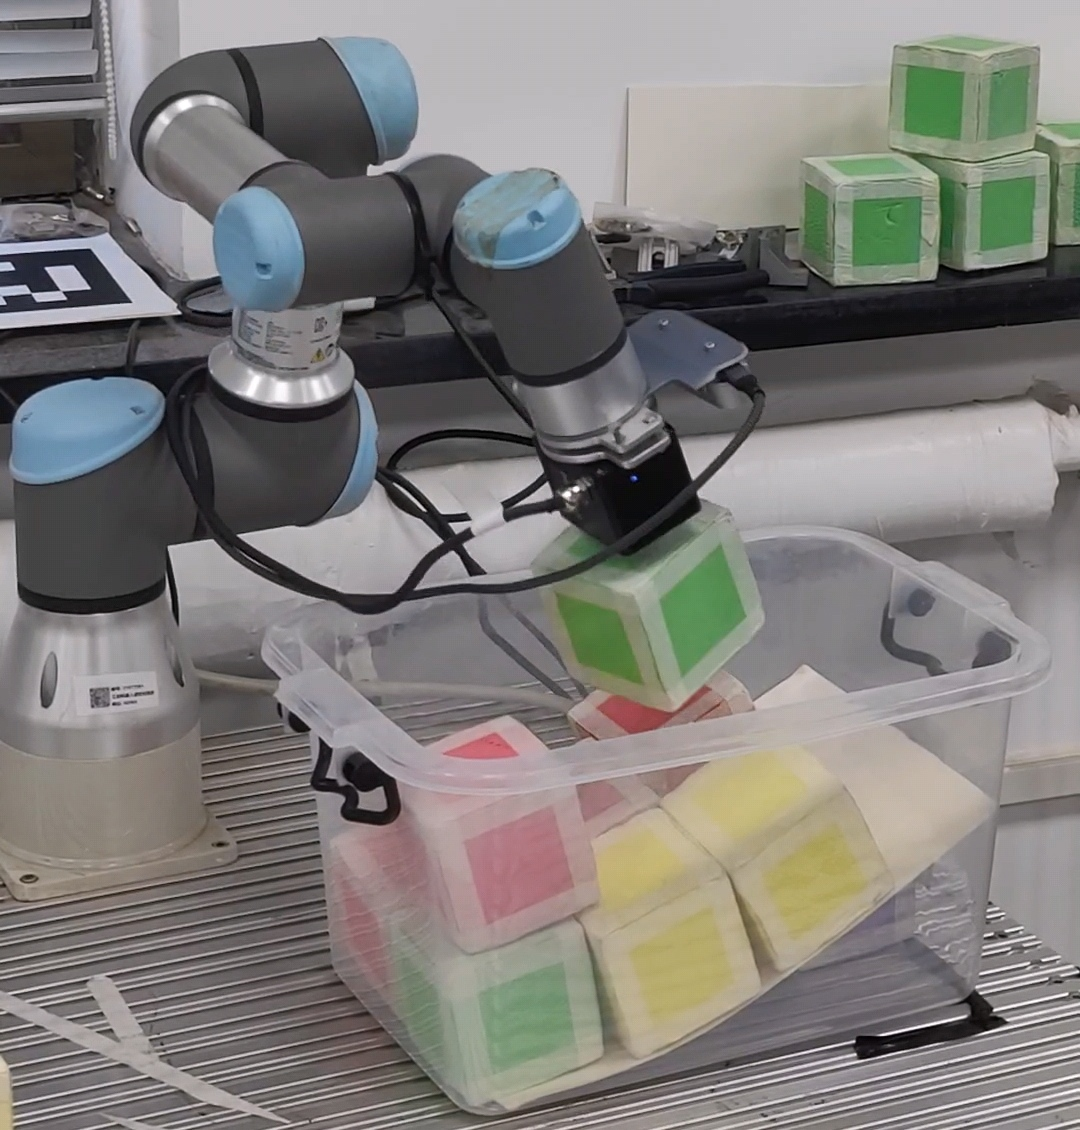
\includegraphics[width=0.99\textwidth]{img/1.jpg}
    \caption{Task~1 抓取过程}
    \label{fig:task1_pick}
  \end{subfigure}
  \hfill
  \begin{subfigure}[b]{0.48\textwidth}
    \centering
    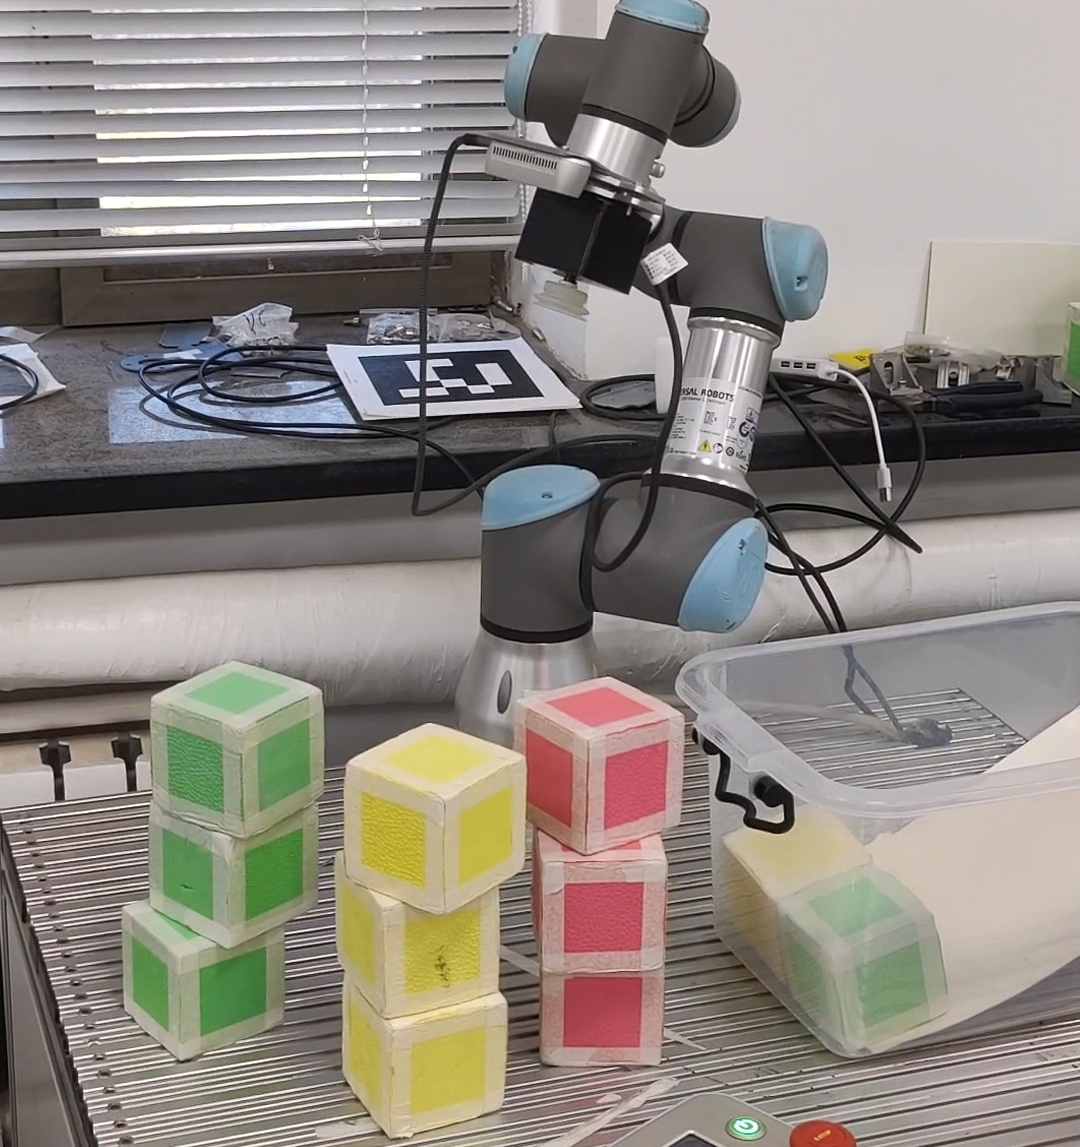
\includegraphics[width=0.99\textwidth]{img/2.jpg}
    \caption{Task~1 堆叠结果}
    \label{fig:task1_stack}
  \end{subfigure}
  \caption{Task~1 比赛过程照片}
  \label{fig:task1_photos}
\end{figure}


\subsection{Task~2 课后自测结果}

比赛结束后，本组自行对 Task~2 进行了功能验证测试，主要结论如下：

\begin{itemize}[noitemsep]
  \item \textbf{轨迹拟合精度}：圆轨迹拟合在转盘匀速旋转时收敛稳定（首次 8~s 采样后），
        预测落点误差在吸盘直径范围内（约 $\leq 15$~mm）；
  \item \textbf{近抓取点修正效果}：实时位姿修正（中心 + 偏航）显著提升了成功率，相比纯预测模式成功率提升约 30\%；
  \item \textbf{层高推算精度}：3 层以上堆叠时，深度估算与真实值误差 $<3$~mm，放置稳定；
  \item \textbf{最大堆叠层数}：测试验证最高可连续堆叠 \textbf{10 块}红色方块
        （\texttt{stack\_max\_level = 10}），受限于机械臂工作空间与堆叠稳定性，10 层为实际安全上限。
\end{itemize}

\begin{figure}[H]
  \centering
  \begin{subfigure}[b]{0.48\textwidth}
    \centering
    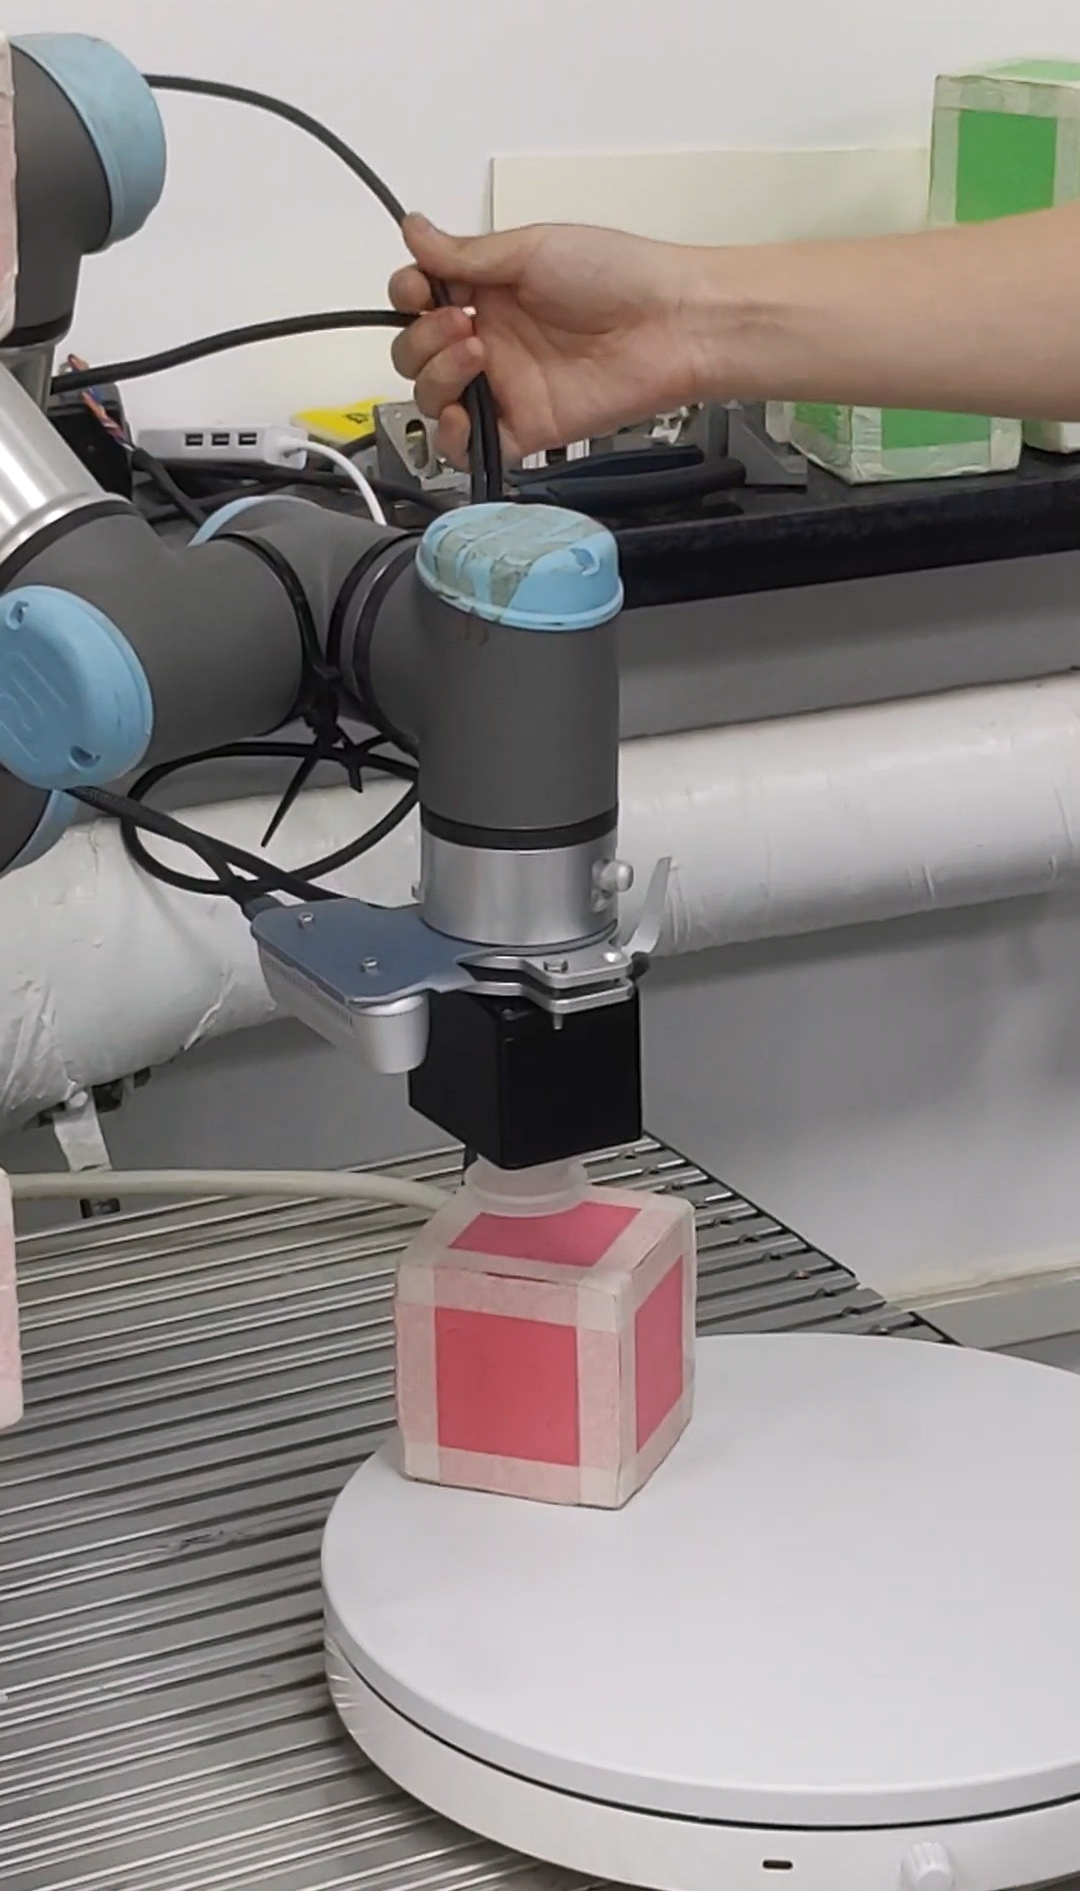
\includegraphics[width=0.9\textwidth]{img/3.jpg}
    \caption{Task~2 动态抓取过程}
    \label{fig:task2_pick}
  \end{subfigure}
  \hfill
  \begin{subfigure}[b]{0.48\textwidth}
    \centering
    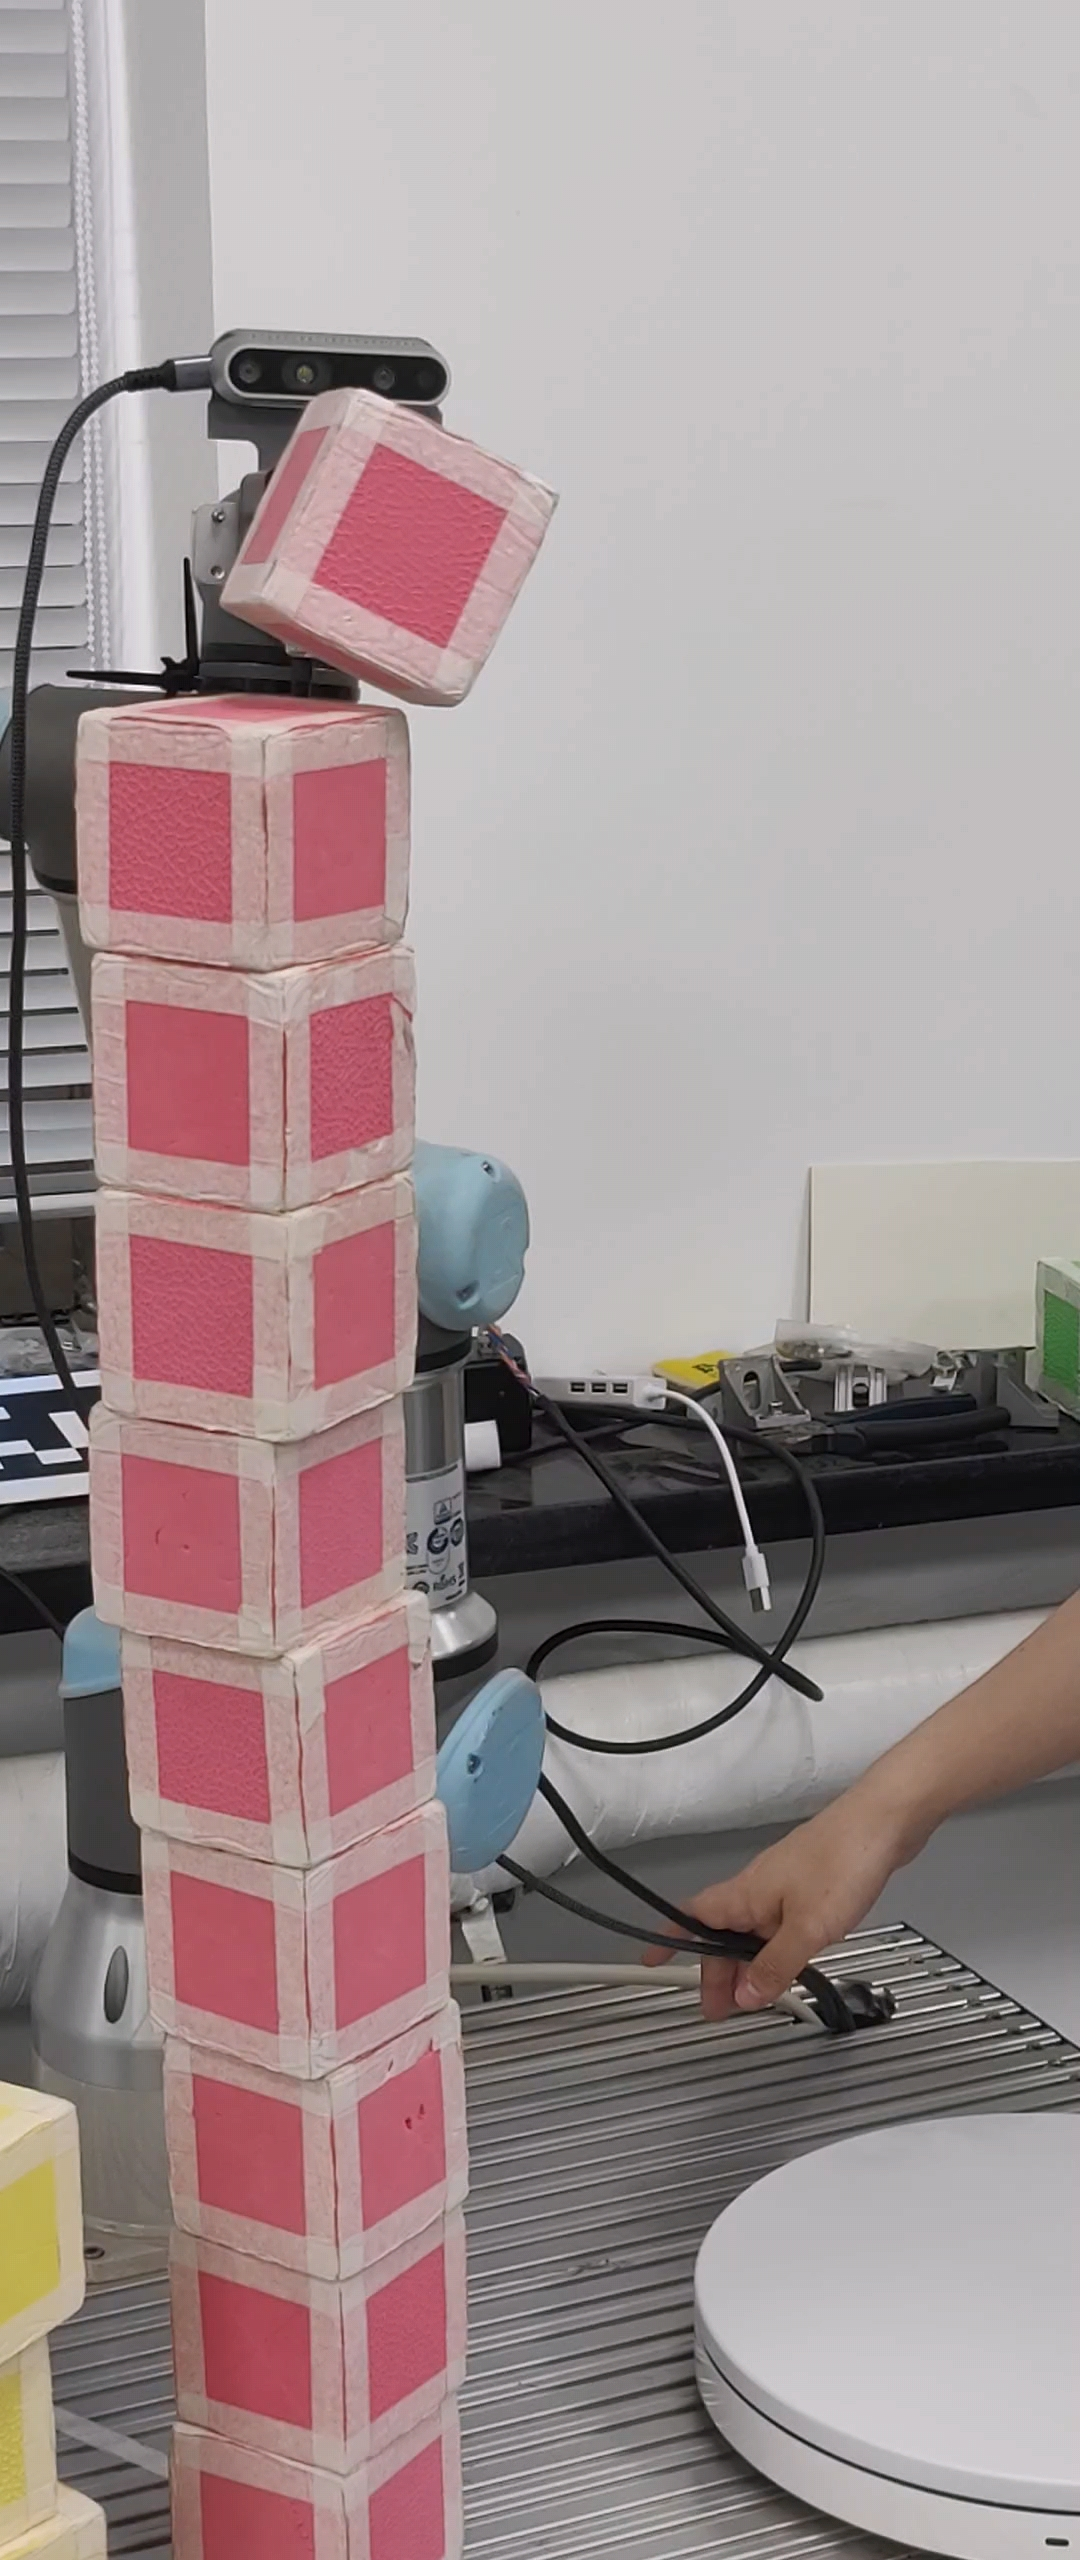
\includegraphics[width=0.68\textwidth]{img/4.jpg}
    \caption{10 块红色方块堆叠结果}
    \label{fig:task2_stack}
  \end{subfigure}
  \caption{Task~2 课后自测照片}
  \label{fig:task2_photos}
\end{figure}

\noindent\textbf{附件视频：}完整的 Task~2 自测过程录像见附件（\texttt{task2\_demo.mp4}）。
视频展示了机械臂从转盘上连续抓取红色方块并逐层堆叠至 10 层的完整流程。

% =============================================================================
\section{结论}
% =============================================================================

本实验实现了基于 ROS~2 的两阶段机械臂抓放系统，主要贡献如下：

\begin{enumerate}[noitemsep]
  \item \textbf{Task~1} 利用 HSV 颜色检测与三维点云反投影，实现了对静态彩色方块的稳定识别与精确拾取；
        通过渐速下降（4 段线性减速至 40\%）、偏航补偿和视觉核验机制提高了放置可靠性；
        比赛中成功完成 9 个方块的分色堆叠，得分 9/16 分。

  \item \textbf{Task~2} 提出了基于最小二乘圆轨迹拟合与线性相位预测的动态目标抓取方案，
        在接近阶段通过实时视觉反馈进一步修正位置和偏航姿态；
        课后自测验证了最高 10 层红色方块的堆叠能力。

  \item \textbf{Launch 文件} 通过 \texttt{OnProcessExit} 事件处理器实现了两阶段任务的无缝衔接；
        所有关键参数可在启动时灵活注入，无需修改源码。
\end{enumerate}

比赛中遭遇的黄色方块凹陷吸附问题，暴露了纯负压吸盘对非平整表面的脆弱性。
\textbf{未来改进方向：}
\begin{itemize}[noitemsep]
  \item 增加吸附力（负压）传感器实时反馈，快速检测吸附失败并自动重试，无需人工干预；
  \item 引入轻量级深度学习目标检测（如 MobileNet-SSD）提升复杂光照下的颜色分割鲁棒性；
  \item 使用卡尔曼滤波或扩展卡尔曼滤波对动态目标进行更精确的轨迹预测，应对转速微小波动；
  \item 优化 Task~1 的单次循环时长（当前约 15--25~s），争取在 5 分钟内同时完成两阶段任务。
\end{itemize}

% =============================================================================
% 附录：核心代码片段
% =============================================================================
\appendix

\section{颜色检测关键代码（Task~1）}
\label{app:color_detect}

\begin{lstlisting}[caption={HSV 颜色掩膜生成（\texttt{\_build\_color\_mask\_from\_hsv}）}]
def _build_color_mask_from_hsv(self, color: str, hsv_image: np.ndarray):
    combined_mask = np.zeros(hsv_image.shape[:2], dtype=np.uint8)
    relax = int(self.color_adaptive_sv_relax)
    for lower, upper in self.color_ranges[color]:
        lower_bound = lower.copy()
        upper_bound = upper.copy()
        if relax > 0:
            lower_bound[1] = np.uint8(max(0, int(lower_bound[1]) - relax))
            lower_bound[2] = np.uint8(max(0, int(lower_bound[2]) - relax))
        combined_mask = cv2.bitwise_or(
            combined_mask, cv2.inRange(hsv_image, lower_bound, upper_bound)
        )
    if self.color_mask_open_iters > 0:
        combined_mask = cv2.morphologyEx(
            combined_mask, cv2.MORPH_OPEN,
            self._color_mask_kernel, iterations=self.color_mask_open_iters,
        )
    if self.color_mask_close_iters > 0:
        combined_mask = cv2.morphologyEx(
            combined_mask, cv2.MORPH_CLOSE,
            self._color_mask_kernel, iterations=self.color_mask_close_iters,
        )
    return combined_mask
\end{lstlisting}

\section{圆轨迹拟合关键代码（Task~2）}
\label{app:circle_fit}

\begin{lstlisting}[caption={最小二乘圆轨迹拟合（\texttt{\_fit\_circle}）与角速度估计（\texttt{\_estimate\_angular\_velocity}）}]
def _fit_circle(self, xy: np.ndarray):
    x = xy[:, 0]
    y = xy[:, 1]
    a = np.column_stack((2.0 * x, 2.0 * y, np.ones_like(x)))
    b = x * x + y * y
    sol, _, _, _ = np.linalg.lstsq(a, b, rcond=None)
    cx, cy, c = sol
    r = np.sqrt(max(1e-9, c + cx * cx + cy * cy))
    return np.array([cx, cy], dtype=np.float64), float(r)

def _estimate_angular_velocity(
        self, t: np.ndarray, xy: np.ndarray, center: np.ndarray):
    rel = xy - center[None, :]
    angles = np.arctan2(rel[:, 1], rel[:, 0])
    angles_unwrapped = np.unwrap(angles)
    t0 = t[0]
    coeff = np.polyfit(t - t0, angles_unwrapped, 1)
    omega = float(coeff[0])
    return omega, float(angles_unwrapped[-1]), float(t[-1])
\end{lstlisting}

\section{位置预测关键代码（Task~2）}
\label{app:predict}

\begin{lstlisting}[caption={目标位置预测与抓取时序控制（\texttt{\_run\_cycle\_once} 节选）}]
# 拟合圆轨迹，首次循环后锁定圆心
fitted_center, radius = self._fit_circle(xy)
center = self._locked_orbit_center_xy.copy()

# 估算角速度
omega, angle_last, t_last = self._estimate_angular_velocity(t, xy, center)

# 预测提前量
dt = float(self.pick_prediction_horizon_sec)
predicted = self._predict_target_position(
    center, radius, angle_last, omega, dt, z_ref
)

# 构建接近/抓取/提升位姿
approach_pose = self._build_tool_pose(
    approach_point, suction_dir,
    camera_z_hint_base=predicted_edge_dir_base
)

# 移动至接近位，精确等待时序对准
approach_start_time = time.monotonic()
self._move_to_pose(approach_pose)
arrive_time = time.monotonic()
t_elapsed = arrive_time - t_last
wait = max(0.0, (dt - self.pick_timing_advance_sec) - t_elapsed)
if wait > 0.0:
    time.sleep(wait)

# 实时修正偏航和中心位置
grasp_pose, lift_pose, delta_yaw, _ = \
    self._refine_grasp_orientation_near_grasp(grasp_pose, lift_pose)
grasp_pose, lift_pose, _ = \
    self._refine_grasp_center_near_grasp(approach_pose, grasp_pose, lift_pose)

# 分阶段旋转下降到抓取位
self._move_approach_to_grasp_with_staged_rotation(
    approach_pose, grasp_pose, delta_yaw
)
\end{lstlisting}

\end{document}
